%----------------------------------------------------------------------------
\chapter{Background} \label{background}
%----------------------------------------------------------------------------

This chapter provides some theoretical background of the contributions presented in this thesis. First of all, the necessary basics of formal language and automaton theory are introduced, afterwards, automaton learning algorithms are discussed.

\section{Basics of automaton theory}

First, we introduce the fundamentals of formal language theory, on which automaton theory is based on. 

\subsection{Fundamentals of formal language theory}
Atomic elements of formal languages are alphabets, characters and words.

\begin{definition}[Alphabet]
	Let $\Sigma$ be a finite, non-empty set. $\Sigma$ is an alphabet, its elements are symbols or characters.
\end{definition}

\begin{definition}[Word]
	If $\Sigma$ is an alphabet, then any finite sequence comprised of the symbols of $\Sigma$ are words (or Strings). $\Sigma^{n}$ represents the set of every $n$ length word consisting of symbols in $\Sigma$: $\Sigma^{n}: w_1w_2\ldots w_n$, where $\forall 0 \leq i \leq n: w_i \in \Sigma$. The set of every word under an alphabet, formally $\bigcup\limits_{n>0}^{} \Sigma^{n}$ is denoted by $\Sigma^{*}$. The empty word is denoted by $\epsilon$.
\end{definition}

Words can be constructed using other words. The following definition defines these relations.

\begin{definition}[Prefixes, Substrings and Suffixes]
	Let an arbitrary $w = uvs$, where $w, u, v, s\in\Sigma^*$. $u$ is the prefix, $v$ is the substring, and $s$ is the suffix of $w$. Formally:
	\begin{itemize}
		\item $w\in\Sigma^*$ is a prefix of $u\in\Sigma^*$ iff $\exists s\in\Sigma^*: s=wu$,
		\item $w\in\Sigma^*$ is a suffix of $u\in\Sigma^*$ iff $\exists s\in\Sigma^*: s=uw$,
		\item $w\in\Sigma^*$ is a substring of $u, v\in\Sigma^*$ iff $u$ is the prefix and $v$ is the suffix of $w$.
	\end{itemize}
\end{definition}

Using these atomic elements of formal language theory, formal languages can be defined.

\begin{definition}[Formal Language]
	An arbitrary set of words under an Alphabet $\Sigma$ is a Language. Formally: $L\subseteq\Sigma^{*}$.
\end{definition}

\begin{definition}[Prefix-closure]
	Let $L\subseteq\Sigma^*$ and $L' = \{u\in\Sigma^*, v\in\Sigma^* : uv\in L\}$. In other words, L' is the set containing all the prefixes of every word of L. L is prefix-closed if $L = L'$.
\end{definition}

Formal language theory is closely linked with automata theory, which we will introduce in the following subsection.

\subsection{Properties of deterministic automata}

Informally, automata are mathematical constructs which read characters from an input and classify them into "accepted" and "rejected" categories. A bit more precisely, automata consist of states, one of which is always active. Starting from an initial state, based on the inputs received, the automaton changes, transitions between states. Essentially, for each of the inputs, the automaton determines whether to keep, or change its current state. In order to determine if an input sequence should be accepted or not, some states are distinguished, accepting states. If after processing a sequence of inputs, the final state of the automaton is an accepting state, the input sequence is accepted. If not, the input is rejected.


One of the most simple automata is the Deterministic Finite Automaton.

\begin{definition}[Deterministic Finite Automaton]
	A Deterministic Finite Automaton is a Tuple of $ DFA=(S,s_{0},\Sigma,\delta,F) $, where: 
	\begin{itemize}
		\item S is a finite, non-epty set containing the states of the automaton,
		\item $s_{0} \in S$ is the initial state,
		\item $\Sigma$ is a finite Alphabet,
		\item $\delta: S\times \Sigma \to S$ is a transition function,
		\item $F\subseteq S$ is a set of the accepting states of the automaton. 
	\end{itemize}
\end{definition}

The deterministic in the name refers to a property of every state having exactly one transition for every input. In other words, every state must have every member of $\Sigma$ listed in its transitions, meaning every state behaves deterministically for every possible input.

An example of a DFA (Deterministic Finite Automaton) from\cite{Steffen2011} can be seen in Example \ref{ex:dfaexample}.

\begin{example}
	\label{ex:dfaexample}
	See Fig. \ref{fig:dfaexample}. This example has four states, $S = \{q_0, q_1, q_2, q_3\}$ (hence $|S| = 4$). The initial state is marked by the start arrow, so $s_0 = q_0$. The alphabet can be inferred as $\Sigma = \{a, b\}$. Transitions are visualized as $q_0$ $\xrightarrow[]{\text{a}}$ $q_1$ given by the transition function (in this example) $\delta(q_0, a) = q_1$. The complete transition function in a table form can be seen in Table \ref{tab:dfaexampledelta}. Finally, the accepting states, or in this case, accepting state of the automaton is $F = \{q_3\}$.
\end{example}
 

The semantics of automata are defined via runs. A run of an automaton is to test for a certain input (word), if it is accepted or rejected. See Example \ref{ex:dfaruns}.

\begin{example}
	\label{ex:dfaruns}
	In accordance with the transition function, a run of Fig. \ref{fig:dfaexample} with an input of $\{a, a, a\}$ would end in state $q_3$ meaning the input is accepted. A rejected input could be $\{a, b, b\}$, which would stop at state $q_1$, a non-accepting state. On deeper examination, one can see, that this automaton only accepts runs with inputs containing $4i+3 a$.
\end{example}

\begin{figure}[H]
	\centering
	\begin{tikzpicture}[shorten >=1pt,node distance=3cm,on grid,auto] 
	\node[state,initial] (q_0)   {$q_0$}; 
	\node[state] (q_1) [right=of q_0] {$q_1$}; 
	\node[state] (q_2) [below=of q_0] {$q_2$}; 
	\node[state,accepting](q_3) [right=of q_2] {$q_3$};
	\path[->] 
	(q_0) edge  node {a} (q_1)
	edge [loop below] node {b} ()
	(q_1) edge  node  {a} (q_2)
	edge [loop below] node {b} ()
	(q_2) edge  node [swap] {a} (q_3) 
	edge [loop above] node {b} ()
	(q_3) edge  node [swap] {a} (q_0)
	 edge [loop above] node {b} () ;
	\end{tikzpicture}
	\caption{A simple DFA from \cite{10.1007/978-3-319-11164-3_26}.}
	\label{fig:dfaexample}
\end{figure}

\begin{table}[H]
\centering
\begin{tabular}{|c|cccc|}
	\hline
	$\delta$ & $q_0$ & $q_1$ & $q_2$ & $q_3$\\ \cline{1-5}
	a & $q_1$ & $q_2$ & $q_3$ & $q_0$ \\	
	b & $q_0$ & $q_1$ & $q_2$ & $q_3$ \\	\hline
\end{tabular}
\caption{The transition function of the automaton seen in Fig. \ref{fig:dfaexample}}
\label{tab:dfaexampledelta}
\end{table}

DFAs are useful to model system behavior based on inputs, but in order to work with reactive systems, we also need to handle outputs. Mealy machines are automata designed to communicate with output symbols instead of accepting and rejecting states.


\begin{definition}[Mealy machine]
	A Mealy machine or Mealy automaton is a Tuple of $ M=(S,s_{0},\Sigma,\Omega,\delta,\lambda) $, where:
	\begin{itemize}
		\item S is a finite, non-empty set containing the states of the automaton,
		\item $s_{0} \in S$ is the initial state,
		\item $\Sigma$ is the input alphabet of the automaton,
		\item $\Omega$ is the output alphabet of the automaton,
		\item $\delta: Q\times \Sigma \to Q$ is the transition function and
		\item $\lambda: Q\times \Sigma \to \Omega$ is the output function. 
	\end{itemize}
\end{definition}

Mealy machines can be regarded as deterministic finite automata over the union of the input alphabet and an output alphabet with just one rejection state, which is a sink, or more elegantly, with a partially defined transition relation. 

An example of a deterministic Mealy machine can be seen in Example \ref{ex:coffeemealy}.

\begin{example}
	\label{ex:coffeemealy}
	An example of a deterministic Mealy machine can be seen in Fig. \ref{fig:coffeemealy}. The formal definition of the automaton can be seen below.
	\begin{itemize} 
		\item $S = \{a, b, c, d, d', e, f\}$ 
		\item $s_0 = a$
		\item $\Sigma = \{water, pod, button, clean\}$
		\item $\Omega$ = \{$\checkmark$, \Coffeecup, $\star$\}
	\end{itemize}
	The transitions, as seen in Fig. \ref{fig:coffeemealy} are visualized as $s_0$ $\xrightarrow[]{\text{input/output}}$ $s_1$, which denotes the machine moving from state $s_0$ to state $s_1$ on the specified input, while causing the specified output. Also, some simplifications are done, e.g. in this transition: d $\xrightarrow[]{\text{\{water,pod\}/\checkmark}}$ d we see a visual simplification of having both transitions merged to one arrow, this is only for visual convenience. Fig. \ref{fig:coffeemealy} is also a great example of sinks, as seen in state f, the machine accepts anything, and never changes. This is a variation of the accepting state seen in DFAs.
\end{example}

\begin{figure}[H]
	\centering
	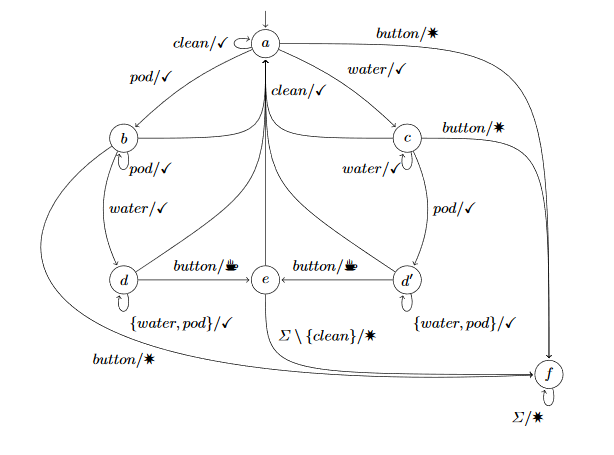
\includegraphics[width=0.7\linewidth]{content/coffeemealy}
	\caption{Mealy machine representing the functionality of a coffee machine.\cite{Steffen2011}}
	\label{fig:coffeemealy}
\end{figure}

Since automaton-based formalisms deal with alphabets, formal language theory is essential not only to define them, but to construct them in a way that is efficient in practical applications. Often automata are used to design and analyze real-life systems. Naturally, questions of efficiency and correctness arise, which is why the relations of automatons and formal languages are discussed more in-depth in the following subsection.

\subsection{Relations of formal languages and automata}

\begin{definition}[Recognized language of automata]
	The language $L\subseteq\Sigma$ containing all the accepted words by an automaton M is called the recognized language of the automaton. It is denoted by L(M) = L.
\end{definition}

\begin{definition}[Regular language]
	A formal language L is regular, iff there is a Deterministic Finite Automaton M, for which L(M) = L, in other words, iff there is a DFA with the recognized language of L.
\end{definition}

Let us now introduce a semantic helper $\delta^*$ for both DFAs and Mealy machines. $\delta^*$ is an extension of the $\delta$ transition function, as $\delta^*: S\times\Sigma^* \to S$ defined by $\delta^*(s,\epsilon) = s$ and $\delta^*(s, \alpha w) = \delta^*(\delta(s, \alpha), w)$, essentially providing the state of the automaton after running an input sequence from a specified state.

\begin{definition}[Myhill-Nerode relation] 
	A DFA $M=(S,s_{0},\Sigma,\delta,F)$ induces the following equivalence relation $\equiv_M$ on $\Sigma^*$ (when L(M) = $\Sigma$):\\
	\null\qquad$x\equiv_M y \iff \delta^*(s, x) = \delta^*(s, y)$\\
	where $x, y\in\Sigma^*$. This means, that x and y are equivalent with respect to $\equiv_M$.\cite{Kozen1977}.
\end{definition}

In words, the Myhill-Nerode relation states, that two words are equivalent wrt. $\equiv_M$ iff runs of both words would end in the same state on the automaton M. The Myhill-Nerode relation is an equivalence relation with some additional properties\cite{Kozen1977}, which can be seen in the following.


\begin{itemize}
	\item The properties of equivalence relations:
	\begin{itemize}
		\item Reflexivity: $x\equiv_M x$.
		\item Symmetry: $x\equiv_M y \implies y\equiv_M x$.
		\item Transitivity: if $(x\equiv_M y$ and $y\equiv_M z) \implies x\equiv_M z$.
	\end{itemize}
	\item Right congruence: $\forall x, y\in\Sigma^*: (x\equiv_M y \implies 		\forall a\in\Sigma: xa\equiv_Mya)$\\ also, by induction, this can be extended to:\\
	$\forall x, y\in\Sigma^*: (x\equiv_M y \implies \forall w\in\Sigma^*: xw\equiv_Myw)$. 
	\item It respects membership wrt. R:\\
	$\forall x, y\in\Sigma^*: x\equiv_M y \implies (x\in R \iff y\in R)$.
	\item $\equiv_M$ is of finite index, has finitely many equivalency classes. Since for every state $s\in S$, the sequences which end up in s are in the same equivalence class, the number of these classes is exactly $|S|$, which is a finite set.
\end{itemize}

Using this relation, we can introduce the Myhill-Nerode theorem, which neatly ties together the previous definitions.

\begin{theorem}[Myhill-Nerode theorem\cite{Kozen1977}\cite{10.2307/2033204}]
	Let $L\subseteq\Sigma^*$. The following three statements are equivalent:
	\begin{itemize}
		\item L is regular.
		\item there exists a Myhill-Nerode relation for L.
		\item the relation $\equiv_L$ is of finite index.
	\end{itemize}
	For proof, see \cite{Kozen1977}\cite{10.2307/2033204}.
\end{theorem}

The same concepts can be applied to Mealy machines, which are somewhat more complex in this regard. As before, a semantic helper is needed similar to $\delta^*$, but considering the output function of Mealy machines. $\lambda^*: S\times\Sigma^* \to \Omega$, defined by $\lambda^*(s, \epsilon) = \varnothing$ and $\lambda^*(s, w\alpha) = \lambda(\delta^*(s, w), \alpha)$.



When monitoring the behavior of Mealy machines, one of the most important metrics given an input is the specific output given by the input. The behavior of a Mealy machine, a specific run of it, has a pattern of \textit{$i_1,o_1,i_2,o_2,..,i_n,o_n$}, where \textit{i} are inputs and \textit{o} are outputs. In order to characterize these runs, we actually do not need every output from this pattern, we only need the final one. Also note, that essentially the final output of a run is given by $\lambda^*(s_0, inputs)$. Let us introduce a $\llbracket M\rrbracket$: $\Sigma^*\to\Omega$ semantic functional as  $\llbracket M\rrbracket(w) = \lambda^*(s_0, w)$. This provides the final output given by a run of an automaton for an input sequence $w$. Using $\llbracket M\rrbracket$, the behavior of Mealy machines can be captured, as discussed in the following.

\begin{example}
	Given the Mealy machine $M\textsubscript{coffeemachine}$ in Fig. \ref{fig:coffeemealy}, the runs:\\
	\null\qquad<clean, $\checkmark$>, \\
	\null\qquad<pod water button, \Coffeecup> \\
	are in $\llbracket M\textsubscript{coffeemachine}\rrbracket$, since the given input words cause the corresponding outputs, while the runs\\
	\null\qquad<clean, \Coffeecup> and \\
	\null\qquad<water button button, $\checkmark$> \\
	are not, since these input sequences do not produce those outputs.
\end{example}

Similarly to the Myhill-Nerode relations in DFAs, equivalence relations over the $P: \Sigma^*\to\Omega$ functional can be introduced, where P is an abstraction of  $\llbracket M\rrbracket$ that can be applied to any state, rather than just the initial state.

\begin{definition}[Equivalence of words wrt. $\equiv_P$\cite{Steffen2011}]
	Given a Mealy machine $M=(S,s_{0},\Sigma,\Omega,\delta,\lambda) $, two words, $u, u'\in\Sigma^*$ are equivalent with respect to $\equiv_P$:\\
	$u \equiv_P u' \iff (\forall v\in\Sigma^*:P(s, uv) = P(s, u'v))$.\\
	We write [u] to denote the equivalence class of u wrt. $\equiv_P$.
\end{definition}

This definition is more along the lines of the right congruence property observed in the Myhill-Nerode relations. The original formalism: $u \equiv_P u' \iff P(s, u) = P(s, u')$ of the Myhill-Nerode relation still stands as a special case of the above definition: if $v=\epsilon$ and $v'=\epsilon$, $P(s, uv) = P(s, u)$ and $P(s, u'v) = P(s, u')$.

\begin{example}
	Taking Fig. \ref{fig:coffeemealy} as an example, the following words are equivalent wrt. $\equiv_{\llbracket M\rrbracket}$:\\
	\null\qquad\qquad\qquad\qquad\space $water, pod$\\
	\null\qquad\qquad$\equiv_{\llbracket M\rrbracket}$\qquad $water, water, pod$\\
	\null\qquad\qquad$\equiv_{\llbracket M\rrbracket}$\qquad $pod, pod, water$.
	
	The first two of $\equiv_{\llbracket M\rrbracket}$ are straightforward, since both words lead to the same state, $d'$, while the third input ends in state $d$. Observably, state $d$ and $d'$ wrt. outputs operate exactly the same regardless of continuation, hence the equivalence holds.
\end{example}

\begin{theorem}[Characterization theorem\cite{Steffen2011}]
	Iff mapping $P: \Sigma^*\to\Omega$ $\equiv_P$ has finitely many equivalence classes, there exists a Mealy machine M, for which P is a semantic functional.
	\\\\
	\textit{Proof}($\impliedby$): As seen in the case of the Myhill-Nerode finite index property for DFAs, same states in Mealy machines will obviously be in same equivalence classes. This implies, that the number of classes in (or in other words, the index of) $\equiv_P$ is at most the number of states the Mealy machine contains, which is finite by definition.
	\\
	\textit{Proof}($\implies$): Consider the following Mealy machine: $M_P=(S,s_{0},\Sigma,\Omega,\delta,\lambda)$:\\
	\null\qquad -S is given by the equivalence classes of $\equiv_P$.\\
	\null\qquad -$s_0$ is given by $[\epsilon]$.\\
	\null\qquad -$\delta$ is defined by $\delta([u], \alpha) = [u\alpha]$.\\
	\null\qquad -$\lambda$ is defined by $\lambda([u], \alpha) = o$, where $P(u\alpha) = o$.\\
	A Mealy machine constructed this way fulfills what the theorem states, P is a semantic functional of it, in other words, $\llbracket M\rrbracket$ = P.
\end{theorem}

With this theorem, regularity for mappings $P:\Sigma^*\to\Omega$ can be defined. A $P:\Sigma^*\to\Omega$ mapping is regular, iff there is a corresponding Mealy machine for which $\llbracket M\rrbracket$ = P, or equivalently, if P has a finite number of equivalence classes, analogously to the previously seen "classical" regularity.

\subsection{Minimization of automata}

The introduction of regularity is useful in the construction of automata, specifically, the construction of canonical automata. 


\begin{figure}
	\centering
	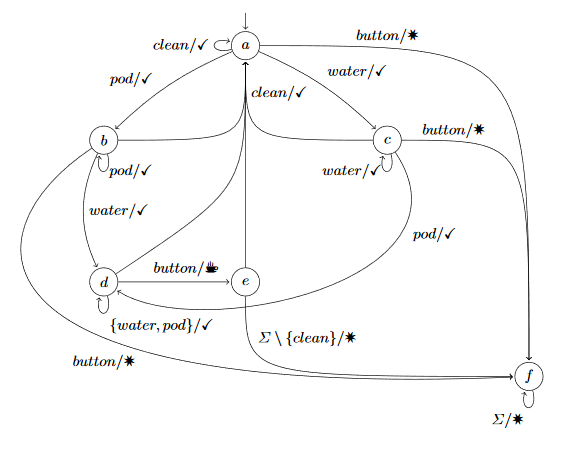
\includegraphics[width=0.7\linewidth]{include/coffeemealyminimal}
	\caption{Minimal version of the Mealy machine seen in \ref{fig:coffeemealy}}
	\label{fig:coffeemealyminimal}
\end{figure}


\begin{definition}[Canonical automaton (Minimal automaton)]
	An automaton M is canonical (i.e. minimal) iff:
	\begin{itemize}
		\item every state is reachable: $\forall s\in S: \exists w\in\Sigma^*: \delta^*(s_0, w) = s$,
		\item all states are pairwisely separable, in other words behaviorally distinguishable. For Mealy machines, this is formalized as: $\forall s_1, s_2\in S: \exists w\in\Sigma^*: \lambda(s_1, w)\neq\lambda(s_2, w)$
	\end{itemize}
\end{definition}

The minimal version of the Mealy machine in Fig. \ref{fig:coffeemealy} can be seen in Fig. \ref{fig:coffeemealyminimal}.


Constructing automata to be canonical, especially in the case of Mealy machines is important with regards to efficiency and is the backbone of automaton learning. The next proposition comes straightforward from the previously presented characterization theorem.


\noindent \textbf{Proposition (Bounded reachability\cite{Steffen2011})}: Every state of a minimal Mealy machine with n states has an access sequence, i.e., a path from the initial state to the given state,  of  length  at  most n-1.  Every  transition  of the model can be covered by a sequence of length at most n from the initial state.

The process of constructing automata uses the concept of partition refinement. It works based on distinguishing suffixes, suffixes of words which mark, witness the difference between two access sequences. The following notion is introduced to formalize this.


\begin{definition}[k-distinguishability\cite{Steffen2011}]
	Two states, $s,s'\in S$ are k-distinguishable iff there is a word $w\in\Sigma^*$ of length k or shorter, for which $\lambda^*(s, w)\neq\lambda^*(s',w)$.
\end{definition} 

\begin{definition}[exact k-distinguishability]
	Two states, $s,s'\in S$ are exact k-distinguishable, denoted by $k^=$ iff s and s' are k-distinguishable, but not (k-1)-distinguishable
\end{definition}

Essentially, if two states, s and s' are  k-distinguishable, then when processing the same input sequence, from some suffix of the word w with length at most k, they will produce differing outputs. Using this, we can observe, that whenever two states, $s_1, s_2\in S$ are (k+1)-distinguishable, then they each have a successor $s_1'$ and $s_2'$ reached by some $\alpha\in\Sigma$, such that $s_1'$ and $s_2'$ are k-distinguishable. These successors are called $\alpha$-successors. This suggests, that:
\begin{itemize}
	\item no states are 0-distinguishable and
	\item two states $s_1$ and s2 are (k+1)-distinguishable iff there exists an input symbol $\alpha\in\Sigma$, such that $\lambda(s_1, \alpha) \neq \lambda(s_2,\alpha)$ or $\delta(s_1, \alpha)$ and $\delta(s_2, \alpha)$ are k-distinguishable.\cite{Steffen2011}
\end{itemize}
This way, if we have an automaton M, we can construct its minimal version, by iteratively computing k-distinguishability for increasing k, until stability, that is until the set of exactly k-distinguishable states is empty.

\begin{example}
	Given the Mealy machine seen in Fig.\ref{fig:coffeemealy}, we can use k-distinguishability to refine its partitions. The initial state, the initial partition would be:\\
	$P_1 = \{a, b, c\}, \{d, d'\}, \{e\}, \{f\}$\\
	since when k=1, a, b and c are not 1-distinguishable, but d and d' separate on the behavior of the \textit{button} input, while e and f are separated by the suffix \textit{clean}. Let's see the k=2 scenario.\\
	$P_2 = \{a\}, \{b\}, \{c\}, \{d, d'\}, \{e\}, \{f\}$\\
	Here, \textit{water} and \textit{pod} separate a, b and c, while d and d' can still no longer be separated. If observed, even if k is increased, d and d' can not be refined. This means, that they are indistinguishable, they can be merged together without altering behavior. This shows the process of acquiring the minimal machine seen in Fig. \ref{fig:coffeemealyminimal}.
	\label{ex:partitionrefinement}
\end{example} 

The process explained in Example \ref{ex:partitionrefinement} is partition refinement, the exact algorithm and proof of its validity can be seen in \cite{Steffen2011}. Partition refinement is a version of the minimization algorithm for DFAs proposed by Hopcroft\cite{HOPCROFT1971189}. 

Let us define one last relation which will be useful in the next section to compare automata minimization and automata learning.

\begin{definition}[k-epimorphisms]
	Let $M=(S,s_{0},\Sigma,\Omega,\delta,\lambda)$ and $M=(S',s_{0}',\Sigma,\Omega,\delta',\lambda')$ be two Mealy machines with shared alphabets. We call a surjective function $f_k: S \to S'$ existential k-epimorphism between $M$ and $M'$, if for all $s'\in S', s\in S$ where $f_k(s) = s'$ and with any $\alpha\in\Sigma$, we have: $f_k(\delta(s,\alpha)) = \delta'(s',\alpha)$, and all states, that are mapped by $f_k$ to the same state of $M'$ are not k-distinguishable.
\end{definition}

 It is straightforward to establish that all intermediate models arising during the partition refinement process are images of the considered Mealy machine under a k-epimorphism, where k is the number of times all transitions have been investigated.\cite{Steffen2011} Essentially this establishes $P_1$ and $P_2$ from Example \ref*{ex:partitionrefinement} as images of the Mealy machine seen in Fig. \ref{ex:coffeemealy} under k-epimorphisms where k=1 and k=2 respectively.

Active automaton learning algorithms operate in a similar way, but they do not have access to the automata they are learning.



\section{Automaton learning}



\paragraph{Automaton learning}  is a way of modeling a system without having specific knowledge of its internal behavior. To accomplish this, the external behavior of the system needs to be observed. This learned model is, as the name suggests, an automaton. 
\\Formally: Automata  learning is  concerned  with  the  problem  of  inferring  an automaton model for an unknown formal language $L$ over some alphabet $\Sigma$\cite{Howar2018}.
\\\\In order to monitor a system, access to its behavioral information is required. There are two approaches, which separate the two types of automaton learning.

\paragraph{Passive automaton learning} In case of passive automaton learning, the gathering of information is not part of the learning process, but rather a prerequisite to it. The learning is performed on a pre-gathered positive an/or negative example set of the systems behavior. In passive automaton learning, the success of the process is determined not only by the efficiency of the algorithm, but the methodology and time used to gather the data.

\paragraph{Active automaton learning} In case of active automaton learning, the behavioral infromation is gathered by the learning algorithm via queries. In order to accomplish this, learning is separated to two components: the learner, which learns, and the teacher, which can answer questions about the system under learning.


Active automaton learning follows the MAT, or the Minimally Adequate Teacher model proposed by Dana Angluin\cite{ANGLUIN198787}. It defines the separation of the algorithm to a teacher and a learner component in a way, where the teacher can only answer the minimally adequate questions needed to learn the system. These two questions, or queries are are follows:


\paragraph{Membership query} Given a $w\in\Sigma^{*}$ word, the query return the $o\in \Omega$ output o corresponding to it, treating the word as a string of inputs. We write $mq(w) = o$ to denote that executing the query w on the system under learning (SUL) leads to the output o: $\llbracket SUL \rrbracket(w) = o$ or $\lambda^*(s_0, w) = o$.

\paragraph{Equivalence query} Given a hypothesis automaton $M$, the query attempts to determine if the hypothesis is behaviorally equivalent to the SUL, and if not, finding the diverging behavior, and return with an example. We write $eq(H) = c$, where $c\in\Sigma^*$, to denote an equivalence query on hypothesis H, returning a counterexample c. The counter example provided is the sequence of inputs for which the output of system under learning and the output of the hypothesis differ: $ \llbracket H\rrbracket(c) \neq mq(c)$.

\noindent The learner component uses membership queries to construct a hypothesis automaton, then refines this hypothesis by the counterexamples provided by equivalence queries. Once counterexamples can not be found this way, the learners hypothesis is behaviorally equivalent to the SUL. The learning can terminate and the output of the learning is the current hypothesis.

\begin{figure}[H]
	\centering
	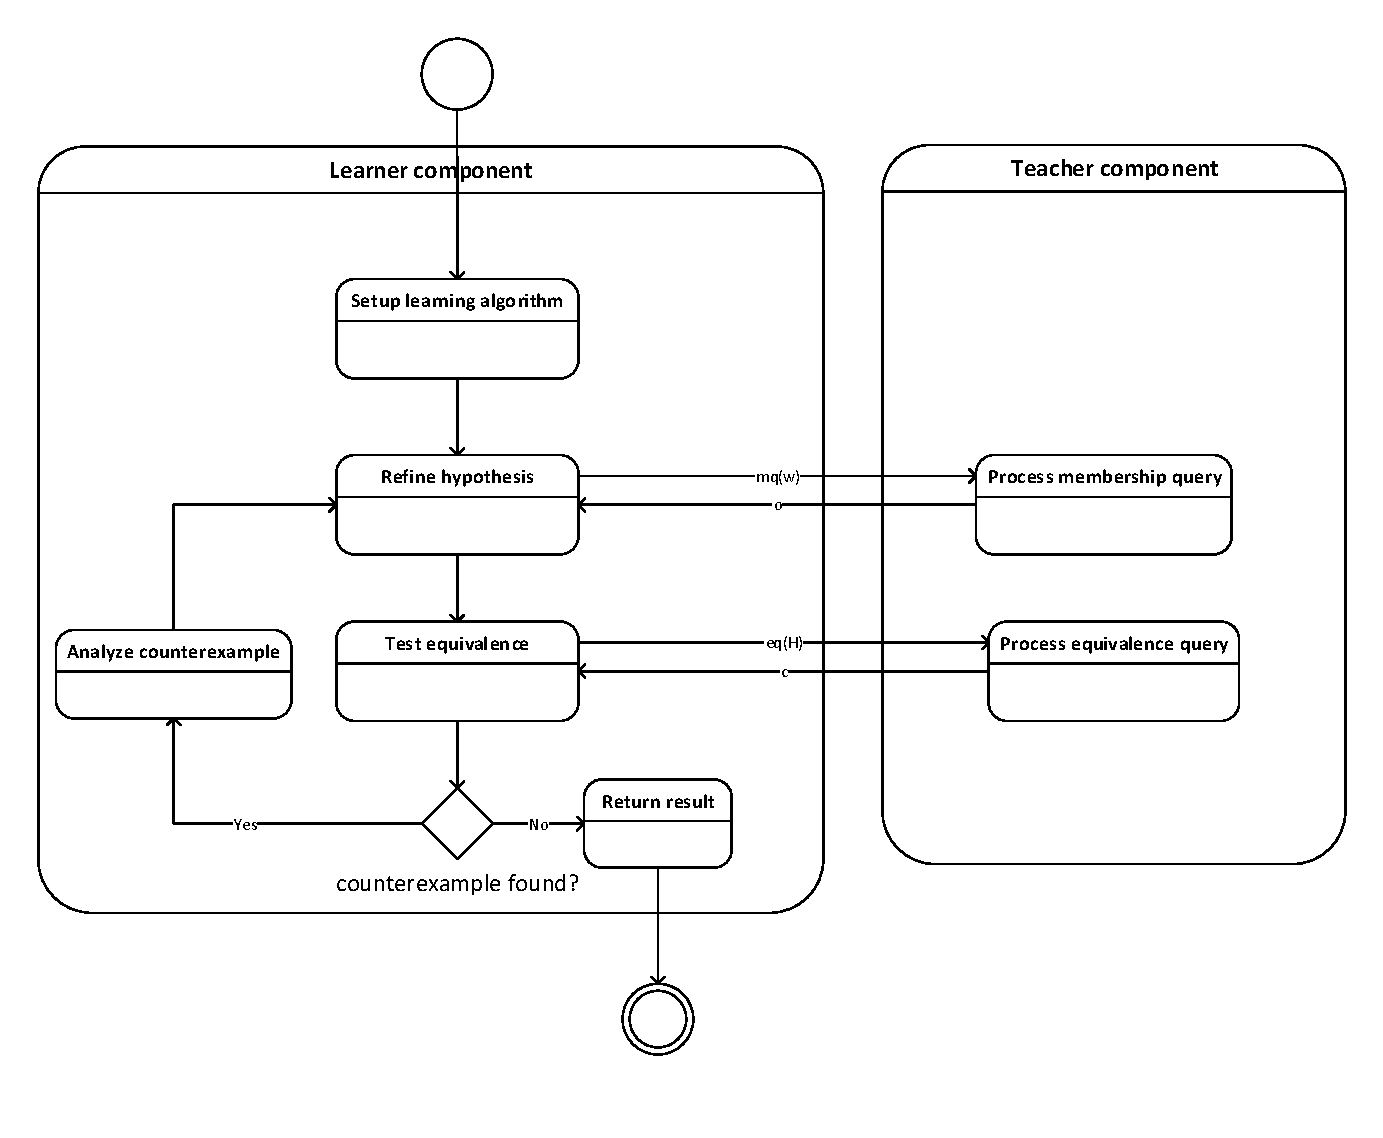
\includegraphics[width=1.0\linewidth]{figures/flowchartlearning}
	\caption{Active automaton learning}
	\label{fig:flowchartlearning}
\end{figure}

As seen on Fig. \ref{fig:flowchartlearning}, the learning proceeds in rounds, generating and refining hypothesis models by exploring the SUL via membership queries. As the equivalence checks produce counterexamples, the next round of this hypothesis refinement is driven by the counterexamples produced.

Using an analogous strategy to the minimization of automata seen in the previous section, starting only with a one state hypothesis automaton, all words are explored in the alphabet in order to refine and extend this hypothesis. Here, there is a dual way of characterizing (and distinguishing) between states\cite{Steffen2011}:
\begin{itemize}
	\item By words reaching them. A prefix-closed set $S_p$ of words, reaching each state exactly once, defines a spanning tree of the automaton. This characterization aims at providing exactly one representative element from each class of $\equiv_P$ on the SUL. Active learning algorithms incrementally construct such a set $S_p$. \\This prefix-closedness is necessary for $S_p$ to be a "spanning tree" of the Mealy machine. Extending $S_p$ with all the one-letter continuations of words in $S_p$ will result in the tree covering all the transitions of the Mealy machine. $L_p$ will denote all the one-letter continuations that are not already contained in $S_p$.
	\item By their future behavior with respect to an increasing vector of words of $\Sigma^*$. This vector $<d_1, d_2,...,d_k>$ will be denoted by $D$, and contains the "distinguishing suffixes". The corresponding future behavior of a state, here given in terms of its access sequence $u\in S_p$, is the output vector$<mq(u*d_1), ..., mq(u*d_k)>\in\Omega^k$, which leads to an upper approximation of the classes of $\equiv_{\llbracket SUL\rrbracket}$. Active learning incrementally refines this approximation by extending the vector until the approximation is precise.
\end{itemize}
While the second characterization defines the states of the automaton, where each output vector corresponds to one state, the spanning tree on $L_p$ is used to determine the transitions of these states. In order to characterize the relation between the SUL $M=(S,s_{0},\Sigma,\Omega,\delta,\lambda)$ and the hypothesis model $M'=(S',s_{0}',\Sigma,\Omega,\delta',\lambda')$ (note, that $M$ and $M'$ only share alphabets), the following definition is introduced. 

\begin{definition}[D-epimorphism]
	Let $D\subseteq\Sigma^*$. We call a surjective function $f_D:S\to S'$ existential D-epimorphism (surjective homomorphism) between $M$ and $M'$ if, for all $s'\in S'$ there exists an $s\in S$ with $f_D(s) = s'$ such that for all $\alpha \in \Sigma$ and all $d\in D$: $f_D(\delta(s, \alpha)) = \delta'(s', \alpha)$, and $\lambda^*(s,d) = \lambda^*(s', d)$. 
\end{definition}

Note, that active learning deals with canonical Mealy machines, in other words, the canonical form of SUL, and not, the perhaps much larger Mealy machine of SUL itself. 

Since active learning algorithms maintain an incrementally growing extended spanning tree for $H=(S_H, h_0, \Sigma, \Omega, \delta_H, \lambda_H)$, i.e., a prefix-closed set of words reaching all its states and covering all transitions, it is straightforward to establish that these hypothesis models are images of the canonical version of SUL under a canonical existential D-epimorphism, where D is the set of distinctive futures underlying the hypothesis construction\cite{Steffen2011}
\begin{itemize}
	\item define $f_D : S_{SUL}\to S_H$ by $f_D(s) = h$ as following: if $\exists w\in S_p \cup L_p$, where $\delta(s_0, w) = s$, then $h = \delta_H(h_0,w)$. Otherwise h may be chosen arbitrarily.
	\item It suffices to consider the states reached by words in the spanning tree to establish the defining properties of $f_D$. This straightforwardly yields:
	\begin{itemize}
		\item $f_D(\delta(s,\alpha)) = \delta_H(h, \alpha)$ for all $\alpha\in\Sigma$, which reflects the characterization from below.
		\item $\lambda^*(s, d) = \lambda^*_H(h,d)$ for all $d\in D$, which follows from the maintained characterization from above.\cite{Steffen2011}
	\end{itemize}
\end{itemize}

In basic logic, D-epimorphisms and k-epimorphisms do not differ, they both deal with establishing constructed models being images of the model they are based on. D-epimorphisms could replace k-epimorphisms where $D=\Sigma^k$, it can be suggested, that there is no need to differentiate. However, there is in important difference of complexity between the two. While k-distinguishability supports polynomial time, black-box systems do not. Also, the "existential" in existential D-epimorphism is important: $f_D$ must deal with unknown states, ones that haven't been encountered yet. This implies that characterization can only be valid for already encountered states.

Active learning algorithms can be proven correct using the following three-step pattern:
\begin{itemize}
	\item Invariance: The number of states of each hypothesis has an upper bound of $\equiv_{\llbracket SUL\rrbracket}$.
	\item Progress: Before the final partition is reached, an equivalence query will provide a counterexample, where an input word leads to a different output on the SUL and on the hypothesis. This difference can only be resolved by splitting at least one state, which increases the state count.
	\item Termination: The refinement terminates after at most the index of $\equiv_{\llbracket SUL\rrbracket}$ many steps, caused directly by the described invariance and progress properties.
\end{itemize}

The following subsection introduces the first active automaton learning algorithm this thesis covers.

\subsection{Direct Hypothesis Construction\cite{10.1007/978-3-642-34781-8_19}}
The Direct Hypothesis Construction algorithm, which hypothesis construction can be seen in Algorithm \ref{algo:dhc}  follows the idea of the breath-first search of graph theory. It constructs the hypothesis using a queue of states, which is initialized with the states of the spanning tree to be maintained. Explored states are removed from this queue, while the discovered successors are enqueued, if they are provably new states. The algorithm starts with a one-state hypothesis, including only the initial state, reached by $\epsilon$ and D = $\Sigma$. It then tries to complete the hypothesis: for every state, the algorithm determines the behavior of the state under D. This behavior is called the extended signature of said state. States with a new extended signatures are provably new states, so to guarantee further investigation, all their successors are enqueued. Initially, $D=\Sigma$, so only the $1^=$-distinguishable states are revealed during the first iteration. This is extended straightforwardly to comprise a prefix closed set of access sequences. \cite{Steffen2011}\cite{10.1007/978-3-642-34781-8_19}

\begin{algorithm}[H]
	\SetAlgoLined
	\DontPrintSemicolon
	\KwIn{$S_p$: a set of access sequences, D: a set of suffixes, an input alphabet $\Sigma$}
	\KwOut{A Mealy machine $H=(S, s_0, \Sigma, \Omega, \delta, \lambda)$}
	initialize hypothesis H, create a state for all elements of $S_p$\;
	initialize a queue Q with the states of H\;
	\While{Q is not empty}{
		s = dequeue state from Q\;
		u = access sequence from $s_0$ to s\;
		\For{$d\in D$}{
			o = mq($u\*d$)\;
			set $\lambda(s,d) = o$\;
		}
		\eIf{exists an $s'\in S$, where the output signature of $s'$ is the same as $s$}{
			reroute transitions of $s$ to $s'$ in H\;
			remove $s$ from H\;
		}{
			create and enqueue successors of $s$ for every input in $\Sigma$ into Q, if not already in $S_p$\;
		}
	}
	Remove entries of $D\setminus\Sigma$ from $\lambda$\;
	\Return{H}\;
	\caption{Hypothesis construction of the Direct Hypothesis Construction algorithm as seen in \cite{Steffen2011}.}
	\label{algo:dhc}
\end{algorithm}

After the execution of the Hypothesis construction seen in Algorithm \ref{algo:dhc}, the output automaton H is used in an equivalence query $eq(H) = c$, to find if a counterexample $c$ exists. If no counteraxamle can be found, the learning terminates, $H$ is the learned automaton. Else, if a counterexample $c$ is found, for which $\lambda_H(s_0,c) \neq mq(c)$, $c$ is used to enlarge the suffixes in D and a new iteration of Algorithm \ref{algo:dhc} begins, using the now extended set D and all the access sequences found in the previous iteration (the current spanning tree $S_p$).

While the DHC algorithm is a straightforward implementation of active automata learning, it struggles with time complexity. It terminates after at most $n^3mk+n^2k^2$ membership queries, and $n$ equivalence queries, where $n$ is the number of states in the final hypothesis, $k$ is the longest set of inputs, and $m$ is the length of the longest counterexample. This renders the DHC algorithm inefficient in practical applications. The next subsection deals with an optimized algorithm, the TTT algorithm.

\subsection{The TTT algorithm\cite{10.1007/978-3-319-11164-3_26}}

As seen in the Direct Hypothesis Construction algorithm, a large number membership queries are required in order to learn an automaton, causing a bottleneck on the scalability of the algorithm. The main cause of this complexity issue is the way counterexamples are treated. In order to ensure every state is properly found, \textit{all} suffixes of the counterexample are added to the algorithms structure, which, has a huge impact on the number of membership queries in the next iteration of the hypothesis construction. TTT resolves this inefficiency by fine-tuning exactly what needs to be further investigated by membership queries.\\\\

\begin{figure}[H]
	\centering
	\begin{subfigure}{0.35\textwidth}
		\centering
		\begin{tikzpicture}[shorten >=1pt,node distance=3.5cm,on grid,auto] 
		\node[state,initial] (q_0)   {$q_0$}; 
		\node[state] (q_1) [right=of q_0] {$q_1$}; 
		\node[state] (q_2) [below=of q_0] {$q_2$}; 
		\node[state](q_3) [right=of q_2] {$q_3$};
		\path[->] 
		(q_0) edge[line width = 0.4mm]  node {a/$\top$} (q_1)
		edge [loop below] node {b/$\top$} ()
		(q_1) edge[line width = 0.4mm]  node[pos=0.62]  {a/$\top$} (q_2)
		edge [loop below] node {b/$\top$} ()
		(q_2) edge[line width = 0.4mm]  node [swap] {a/$\bot$} (q_3) 
		edge [loop above] node {b/$\top$} ()
		(q_3) edge  node[pos=0.62] [swap] {a/$\top$} (q_0)
		edge [loop above] node {b/$\bot$} () ;
		\end{tikzpicture}
		\caption{A Mealy-machine version of the DFA seen in Fig. \ref{fig:dfaexample}.}
	\end{subfigure}
	\begin{subfigure}{0.55\textwidth}
		\centering
		\begin{tikzpicture}[shorten >=1pt,node distance=1.8cm,on grid,auto] 
		\node[state] (e)   {$\epsilon$}; 
		\node[state] (a) [below left=of e] {$a$}; 
		\node[state] (q3) [right=of a] {$q_3$}; 
		\node[state] (aa) [below left=of a] {$aa$};
		\node[state] (q2) [right=of aa] {$q_2$}; 
		\node[state] (q0) [below left=of aa] {$q_0$}; 
		\node[state] (q1) [right=of q0] {$q_1$}; 
		\path[->] 
		(e) edge node {} (a)
		(e) edge node {} (q3)
		(a) edge node {} (aa)
		(a) edge node {} (q2)
		(aa) edge node {} (q0)
		(aa) edge node {} (q1);
		\end{tikzpicture}
		\caption{Final discrimination tree.}
	\end{subfigure}
	\begin{subfigure}{0.2\textwidth}
		\centering
		\begin{tikzpicture}[shorten >=1pt,node distance=1.8cm,on grid,auto] 
		\node[state] (e)   {$\epsilon$}; 
		\node[state] (a) [below=of e] {$a$}; 
		\node[state](aa) [below=of a] {$aa$};
		\path[->] 
		(aa) edge node {a} (a)
		(a) edge node {a} (e);
		\end{tikzpicture}
		\caption{Discriminator trie of the final hypothesis.}
	\end{subfigure}	
	\caption{The three namesake trees of the TTT algorithm, (a) being a spanning \textbf{T}ree, (b) a disctimination \textbf{T}ree, and (c) a discriminator \textbf{T}rie.}
	\label{fig:dfaexamplemealyver}
\end{figure}

\begin{example}
	As an example, we'll use the automaton portrayed on Fig.\ref{fig:dfaexamplemealyver}.a, a Mealy machine version of the DFA previously seen in Fig.\ref{fig:dfaexample} constructed simply by the following rule: if a transition ends in $q_3$, the output is $\bot$, else the output is $\top$.
	\\TTT keeps the notion of separating states by a spanning tree $S_p$, a prefix-closed set of words from $\Sigma^*$, this tree defines the access sequences of each state. The spanning tree $S_p$ is indicated by bold transitions in Fig.\ref{fig:dfaexamplemealyver}.a. 
	\\States are separated by the notion of discriminators. The algorithm maintains a set of discriminator suffixes D, but uses them differently from the DHC algorithm. D in TTT is used by a n-ary tree, where n = $|\Omega|$, so in this example a binary tree. We call this tree a discrimination tree (seen in Fig.\ref{fig:dfaexamplemealyver}.b), which maintains information about which inputs (discriminators) separate states: for every distinct pair of states, a separator can be obtained by looking at the label of the lowest common ancestor of the corresponding leaves. This way, the label of inner nodes act as discriminators. These labels form a suffix-close set and are stored in a trie seen in Fig.\ref{fig:dfaexamplemealyver}.c. Each node of the trie is a word, which can be constructed by going up the tree towards the root.
\end{example}

Discriminator trees, as seen in the previous example, are rooted n-ary trees, where n is the size of the output alphabet. Leaves are labeled by states of the automaton, while inner states are labeled by discriminators (suffixes). When adding a new word to the tree $T$, we sift the word $w\in\Sigma^*$ into T by starting at the root, and for every inner node $v\in D$, we branch depending on the output of $\lambda^*(wu)$. This limits the number of membership queries to the height of the tree, while DHCs limit was $S_p\times D$.
\\\\
\textbf{Key steps of the TTT algorithm:}
\begin{itemize}
	\item \textbf{Hypothesis construction.} The initial state is initialized and membership queried for all inputs, the results of which are sifted into the discriminator tree T.
	\item \textbf{Hypothesis refinement.} If a counterexample is found, the corresponding state is split (analogously to the DHC algorithm), in the discriminator tree, the leaf corresponding to this new state is split by a temporary discriminator $v\in\Sigma$.
	\item \textbf{Hypothesis stabilization.} The hypothesis provided by the previous example might contradict information of the discrimination tree. This step searches for counterexamples between them (without the need of equivalence queries), and if any such counterexample exist, states are split accordingly.
	\item \textbf{Discriminator finalization.} TTT treats discriminators derived directly from counterexamples temporary, keeping track of the maximal sub-tree of the discrimination tree containing temporary discriminators. This sub-tree is split as temporary discriminators are replaced with final ones. Only when this finalization happens, is an inner node of the discrimination tree considered a member of the discriminator trie, in other words, when finalizing a temporary discriminator, it is added to the discriminator trie.
\end{itemize}
For a more detailed description of the TTT algorithm the reader is referred to\cite{10.1007/978-3-319-11164-3_26}.